% !TEX TS-program = pdflatex
%\documentclass[draftcls, onecolumn, journal]{IEEEtran}
\documentclass[journal]{IEEEtran}
%\documentclass[a4paper,11pt]{article}
%\usepackage{fullpage}

%\renewcommand{\baselinestretch}{1.9}
\usepackage[hidelinks]{hyperref}
\usepackage{graphicx}
\usepackage{color}
\usepackage{amsmath}
\usepackage{caption}
%\usepackage{cite}
\usepackage[
style=ieee,
sorting=ynt
]{biblatex}
\graphicspath{images/}
\addbibresource{sources.bib}

\newcommand{\argmax}[1]{\underset{#1}{\operatorname{arg}\,\operatorname{max}}\;}

%\bibliographystyle{IEEEtran}

%%%%%%%%%%%%%%%%%%%%%%%%%%%%%%%%%%%%%%%%%%%%%%%%%%%%%%%%%%%%%%%%%%%%%%
\title{Fan-Beam Computerized Tomography Simulation}

\author{Kutay Ugurlu}

%%%%%%%%%%%%%%%%%%%%%%%%%%%%%%%%%%%%%%%%%%%%%%%%%%%%%%%%%%%%%%%%%%%%%%
\begin{document}
%\renewcommand{\baselinestretch}{1.6}

\maketitle

\begin{abstract}This project report demonstrates the implementation of Fan Beam Computerized Tomography simulation. The effect of different design parameters including the length of the detector, the number of beams and the angle between consecutive projections is inspected and discussed comparatively in both quantitative and qualitative manner. The work is derived from the previously developed code in Parallel Beam X-Ray Computerized Tomography \cite{ugurlu2021}. The developed software and GUI to run it can be found in \href{https://github.com/kutay-ugurlu/Fan-Beam-Computerized-Tomography-Simulation}{github.com/kutay-ugurlu/Fan-Beam-Computerized-Tomography-Simulation} \\
%\textit{Keywords:} Inverse electrocardiography, electrocacardiographic imaging, statistical estimation, Bayesian estimation, Kalman filter.
\end{abstract}
\begin{IEEEkeywords}
	imaging, medical imaging, X-Ray computerized tomography, image reconstruction
\end{IEEEkeywords}

\section{Introduction} \label{sec:intro}
The purpose of this project report is to demonstrate the procedure followed to simulate Fan-Beam Projected X-Ray Computerized Tomography. This project report consists of \nameref{sec:theory}, \nameref{sec:implementation}, \nameref{sec:results} and \nameref{sec:discuss} sections. The second section introduces the technical background for the CT simulation and the following section illustrates the algorithm using pseudocode snippets. \nameref{sec:results} and \nameref{sec:discuss} section presents the comparative results regarding different user-specified parameters with the conclusion and reasons behind them.

\subsection{History}
The history of X-Ray Computerized Tomography can be dated back to 1917, when an Austrian mathematician called Johann Radon invented an algorithm, referred to as Radon transform today, on how to calculate line integrals in a two-dimensional section. The idea of computed tomography was developed in 1967 and was first used in a medical setting was in 1971 \cite{richmond2004sir}, by Godfrey Hounsfield. The device was tested at
James Ambrose’s department at Atkinson Morley Hospital in Wimbledon. This first model did not include a computer, instead the waves was written on a magnetic tape of the device EMI Scanner CT1010. 

\begin{figure}[h]
\centering
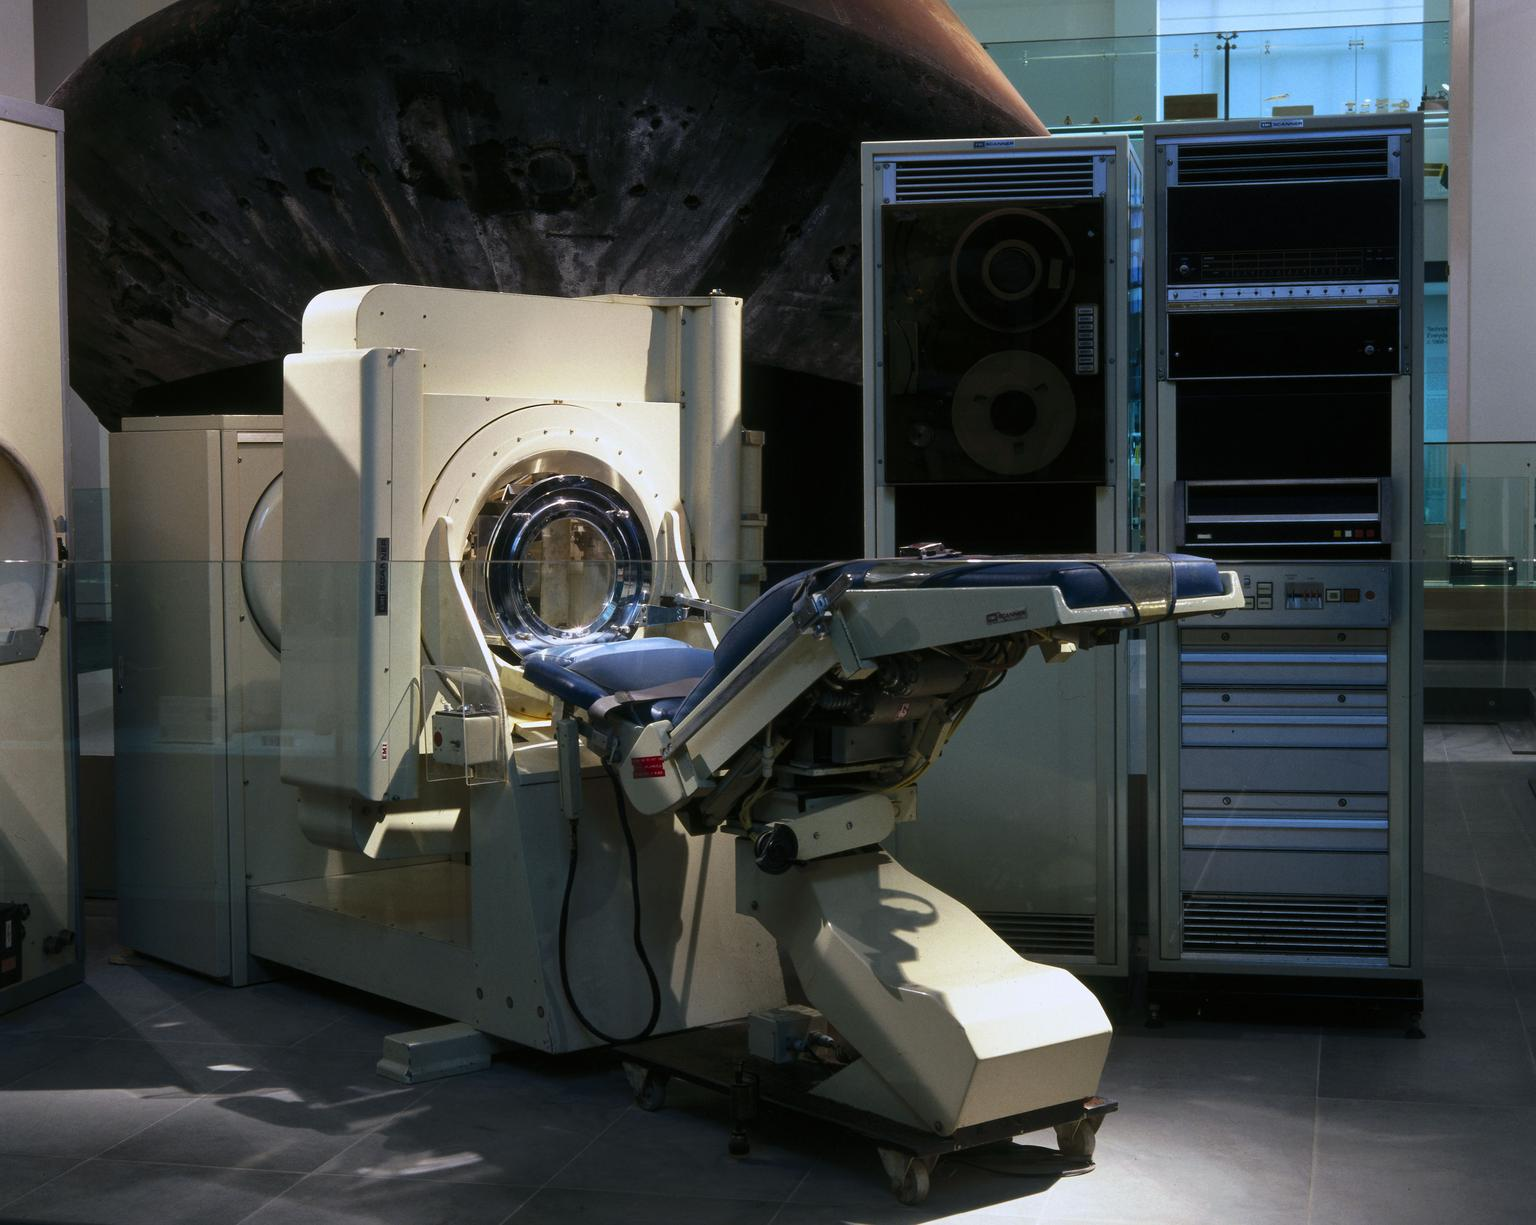
\includegraphics[width=0.3\textwidth]{images/CT.jpg}
\centering \caption{First EMI Scanner \cite{emict}}\label{fig:CT1010}
\end{figure}

\section{Theory} \label{sec:theory}

\section{Implementation} \label{sec:implementation}

\section{Results} \label{sec:results}

\section{Discussion} \label{sec:discuss}

\printbibliography

\end{document}

